\documentclass[../main.tex]{subfiles}

\begin{document}

\section{Observación}

Al calcular el factor de estructura estático $S(q)$ de la red, se observa que a valores pequeños de $q = |\mathbf{q}|$ la curva muestra un decaimiento aparentemente exponencial modulado por oscilaciones de tipo sinusoidal. 
\begin{figure}[ht!]
    \centering
    
\includegraphics[width=0.8\textwidth]{../Figures/may20/fig_Sqcomp_phi_1.0.png}
\end{figure}

\begin{figure}[ht!]
    \centering
    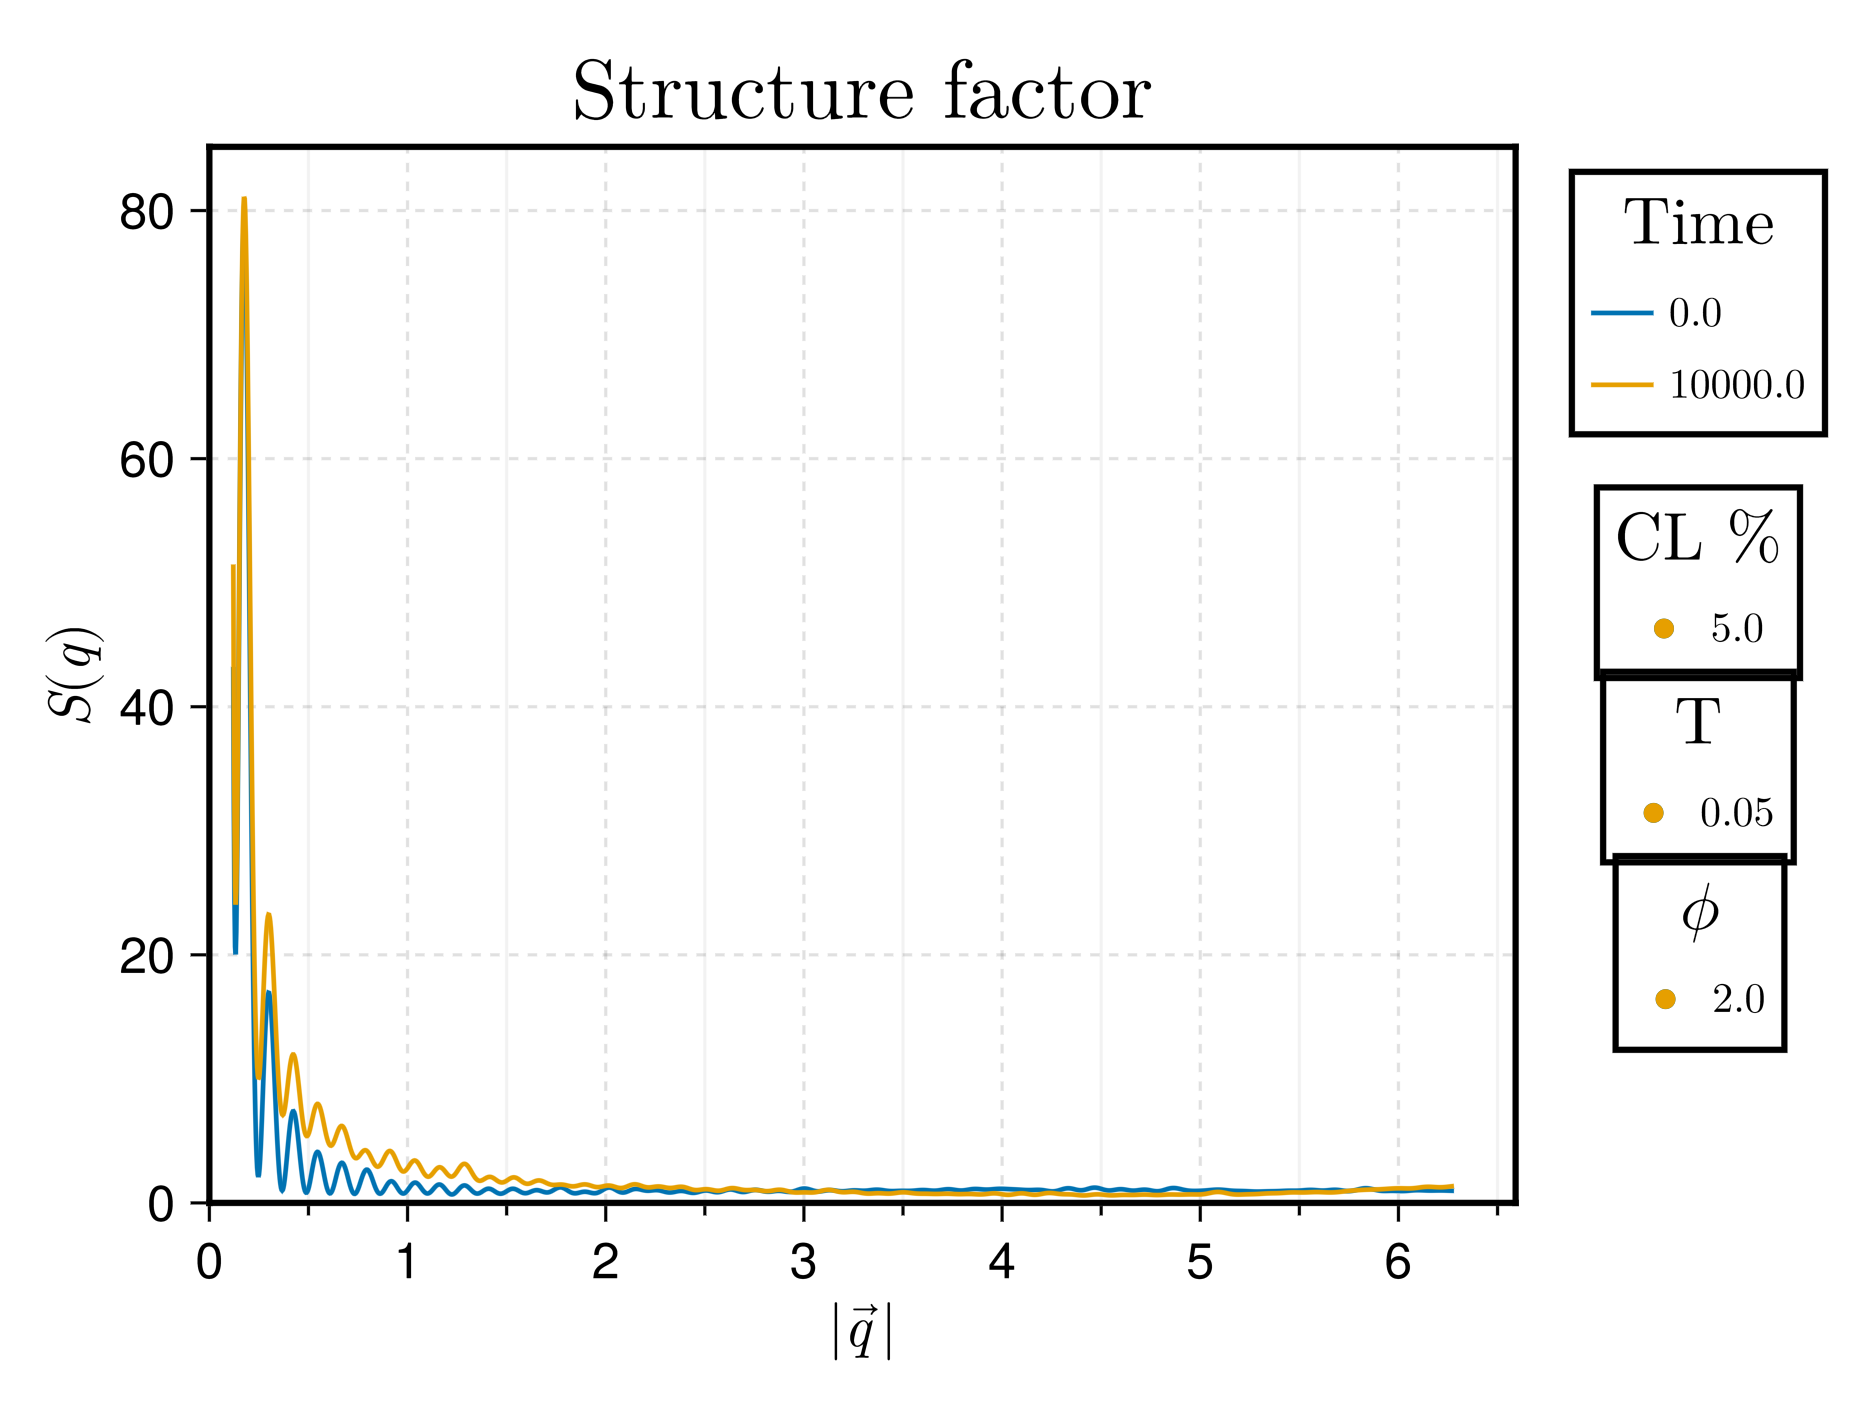
\includegraphics[width=0.8\textwidth]{../Figures/may20/fig_Sqcomp_phi_2.0.png}
\end{figure}

\begin{figure}[ht!]
    \centering
    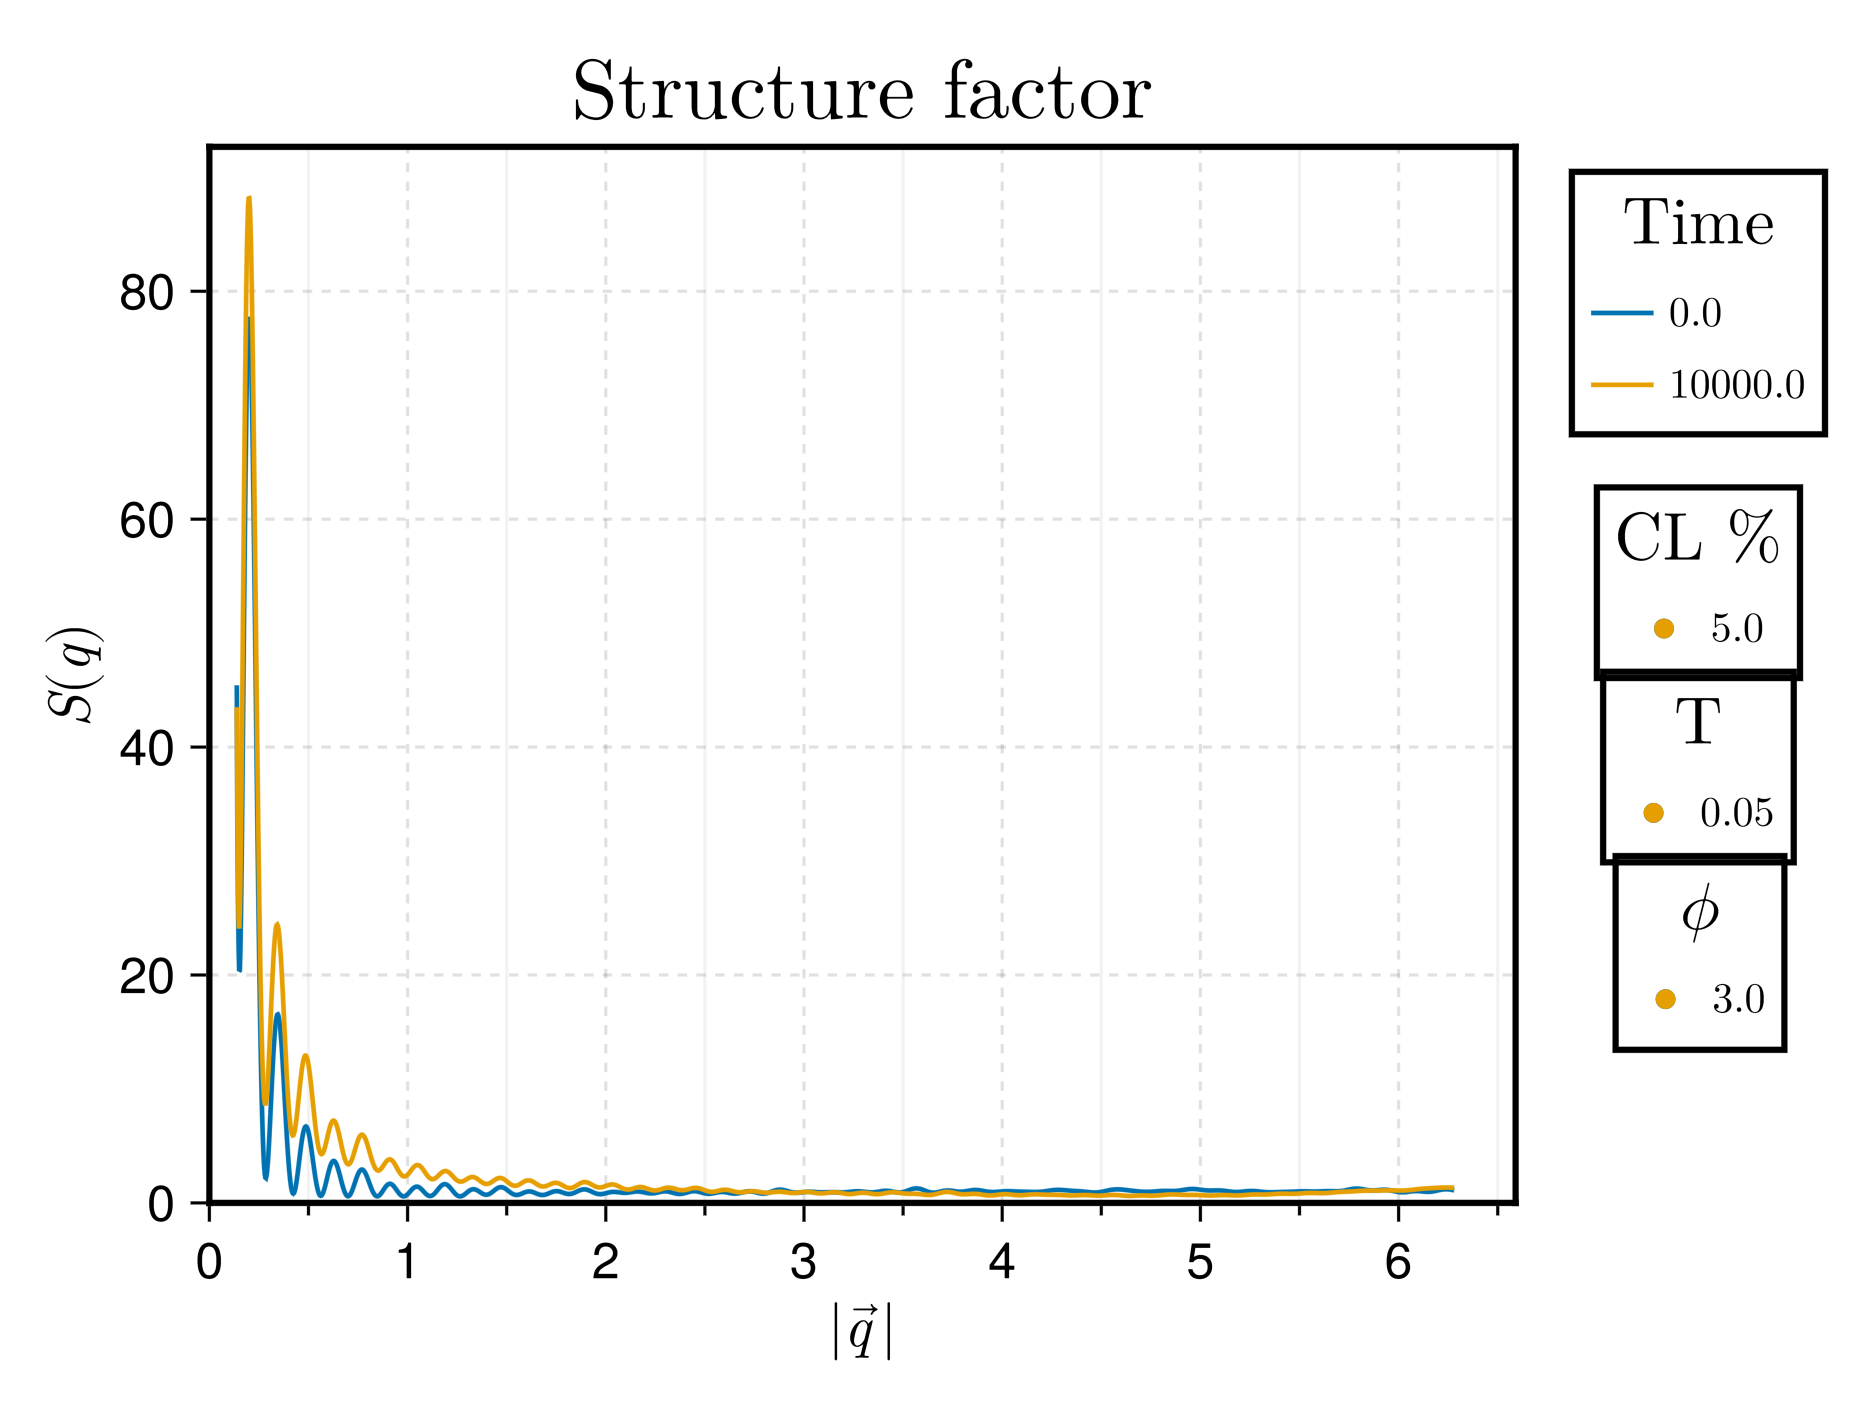
\includegraphics[width=0.8\textwidth]{../Figures/may20/fig_Sqcomp_phi_3.0.png}
\end{figure}

\begin{figure}[ht!]
    \centering
    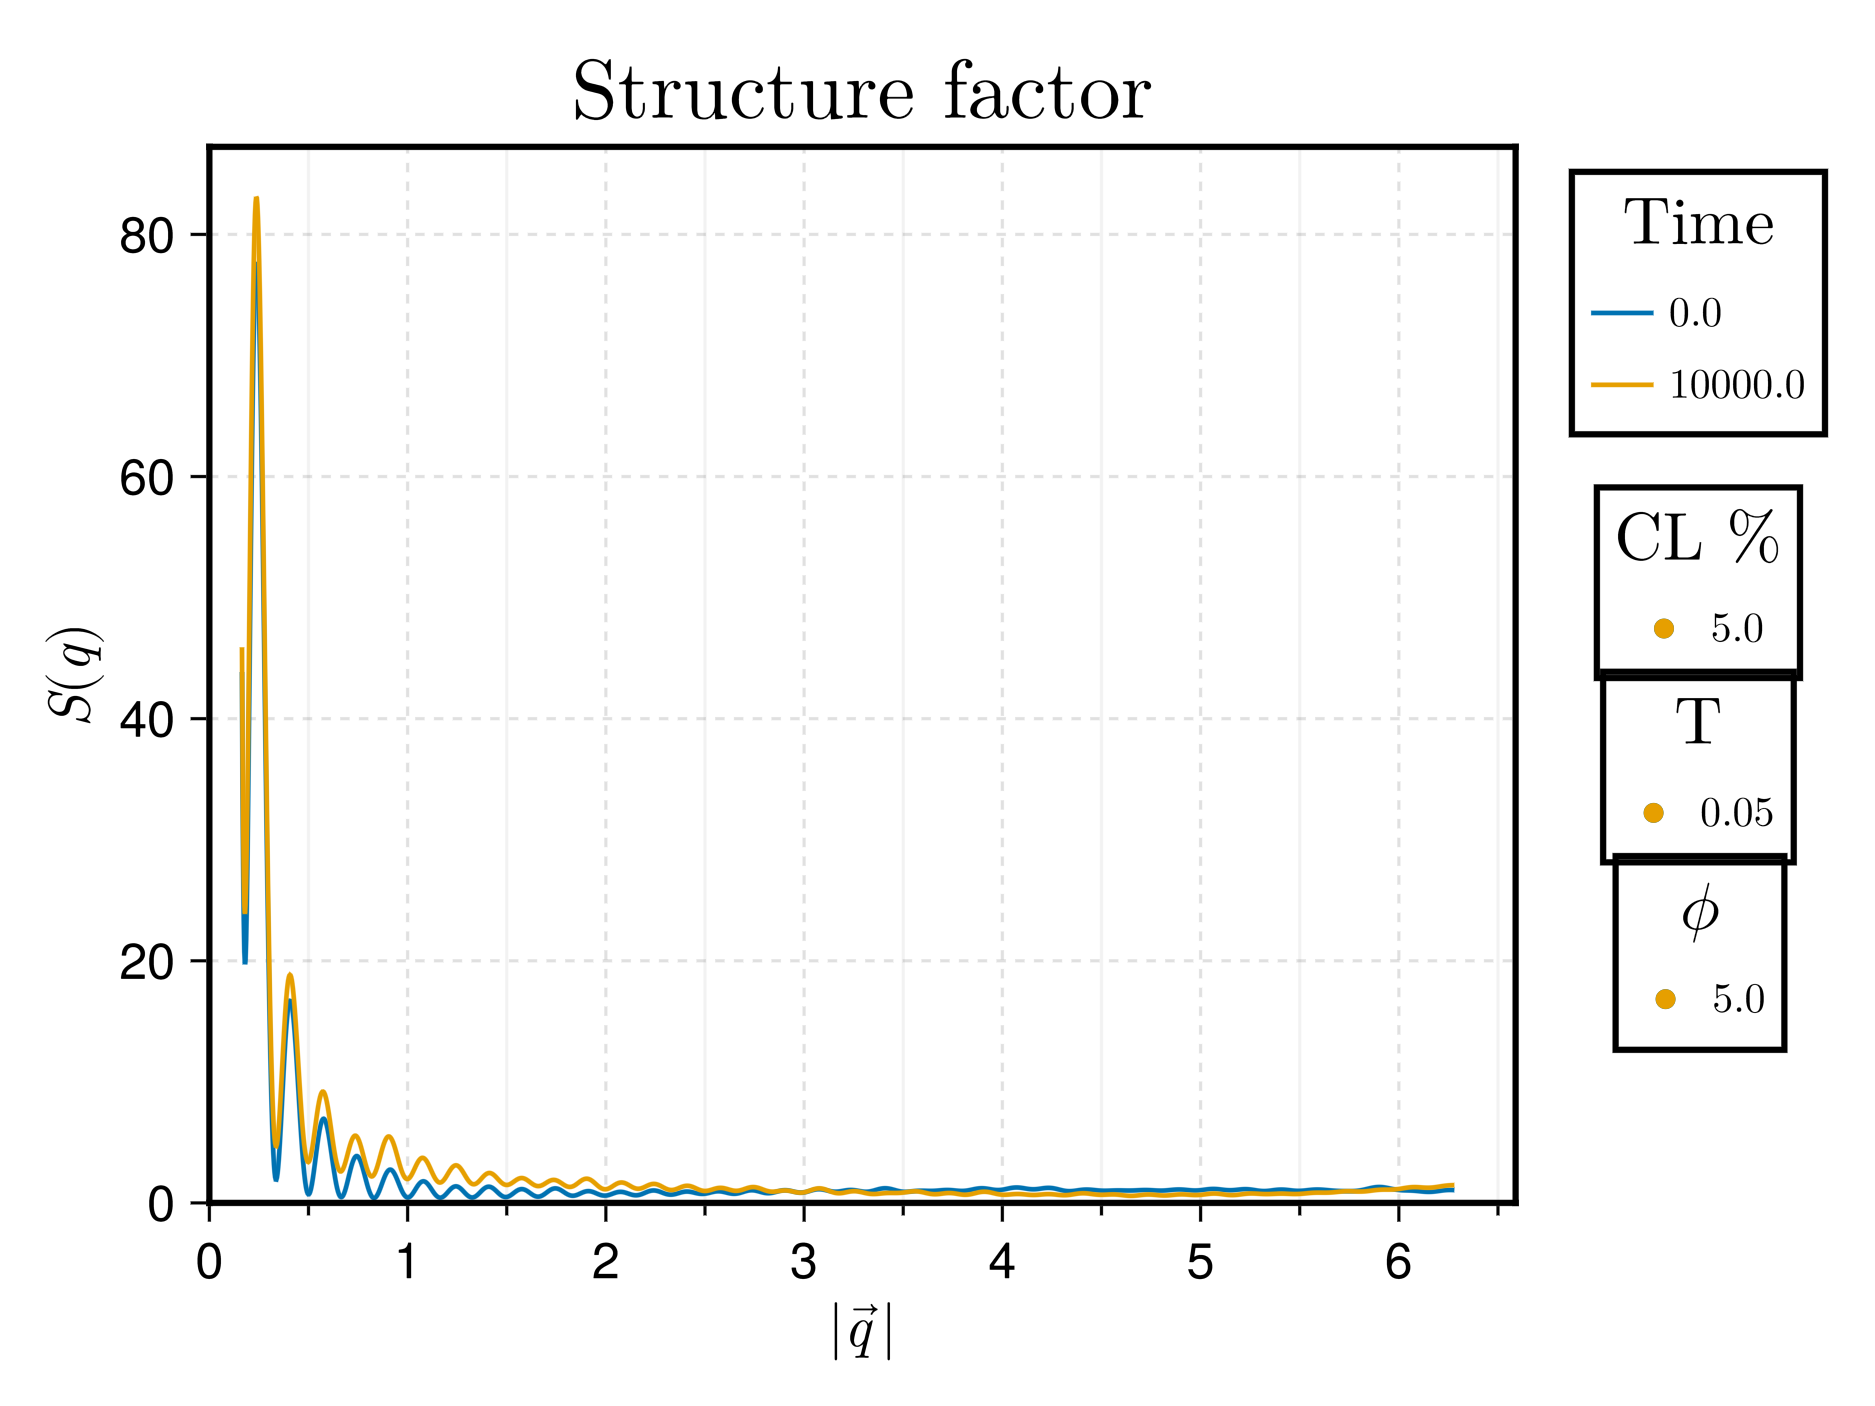
\includegraphics[width=0.8\textwidth]{../Figures/may20/fig_Sqcomp_phi_5.0.png}
\end{figure}

De acuerdo con DeepSeek, este comportamiento no es físico; es un artefacto numérico debido al factor de forma de la caja de simulación.



\section{Origen del artefacto}

En condiciones periódicas de frontera, la densidad microscópica $\rho(\mathbf{r}) = \sum_{j=1}^{N} \delta(\mathbf{r} - \mathbf{r}_j)$ se replica en todo el espacio. Su transformada de Fourier, evaluada en vectores de onda arbitrarios, es
\begin{equation}
\tilde{\rho}(\mathbf{q}) = \sum_{j=1}^{N} e^{-i\mathbf{q}\cdot\mathbf{r}_j} \;
\underbrace{\prod_{\alpha=x,y,z} \frac{\sin(q_\alpha L/2)}{q_\alpha L/2}}_{\text{factor de forma de la caja}},
\label{eq:ff}
\end{equation}
donde $L$ es la longitud de la celda cúbica. El factor de forma es una función $\operatorname{sinc}(q_\alpha L/2)$ que introduce un decaimiento algebraico $\sim 1/q$ y oscilaciones con período $\Delta q \approx 2\pi/L$ en cada dirección. Al promediar angularmente para obtener $S(q)$, estas oscilaciones se manifiestan como una modulación sobre la señal física, particularmente notoria a bajo $q$ donde la longitud de onda $2\pi/q$ es comparable al tamaño de la caja.

\section{Solución: uso exclusivo de vectores recíprocos}

Para eliminar por completo este artefacto, se deben emplear únicamente los vectores de onda que son compatibles con las condiciones periódicas de la celda:
\begin{equation}
\mathbf{q} = \frac{2\pi}{L}(n_x,\, n_y,\, n_z),\qquad n_x,n_y,n_z \in \mathbb{Z}.
\label{eq:qcomp}
\end{equation}
En estos vectores, $q_\alpha L/2 = \pi n_\alpha$ y el factor de forma se anula idénticamente (vale $1$ para $n_\alpha=0$ o se evalúa como $\operatorname{sinc}(\pi n_\alpha) = 0$ para $n_\alpha \neq 0$)\sidenote{En el cálculo de $S(q)$ se toma el módulo cuadrado; para $n_\alpha \neq 0$ el factor de forma es $0$, por lo que esos modos no contribuyen al promedio si el vector posee alguna componente no nula con $n_\alpha \neq 0$. Esto excluye automáticamente los artefactos. La contribución neta de la caja se vuelve exactamente $1$ para los vectores recíprocos permitidos que efectivamente participan.}. Así, el factor de estructura calculado será puramente el de la distribución de partículas dentro de la celda.

En la práctica, se generan los vectores $\mathbf{q}$ definidos por (\ref{eq:qcomp}) hasta una magnitud máxima deseada, y se agrupan por el módulo $q$ para obtener la dependencia radial $S(q)$. Esta restricción elimina por completo las oscilaciones espurias y revela la verdadera forma de $S(q)$ a bajo $q$, típicamente una meseta o un pico ancho correspondiente al tamaño de malla de la red.

\section{Verificación}

Para confirmar que las oscilaciones observadas provenían del factor de forma, se puede repetir el cálculo cambiando el tamaño de la caja $L$: la periodicidad de las modulaciones debe escalar como $2\pi/L$. Una vez aplicada la restricción (\ref{eq:qcomp}), la curva se suaviza y el artefacto desaparece.

\end{document}
